\documentclass[12pt,letterpaper,noanswers]{exam}
\usepackage[usenames,dvipsnames,svgnames,table]{xcolor}
\usepackage[margin=0.9in]{geometry}
\renewcommand{\familydefault}{\sfdefault}
\usepackage{multicol}
\pagestyle{head}
\header{AM 108 Class 22}{}{Lorenz system}
\runningheadrule
\headrule
\usepackage{graphicx} % more modern
\usepackage{amsmath} 
\usepackage{amssymb} 
\usepackage{hyperref}
\usepackage{tcolorbox}

\begin{document}
 \pdfpageheight 11in 
  \pdfpagewidth 8.5in

\noindent 




\begin{itemize}
\item No problem set: project work this week (guidelines posted by tomorrow at noon ET).
\item There is a skill check for Monday.
\item There will be a pre-class assignment for Monday.
\end{itemize}

\hrule
\vspace{0.2cm}



\noindent\textbf{Project Teams}

Team 1:


\noindent \textbf{Teams 5 and 6}: Post screenshots of your work to the course Google Drive today.  Include words, labels, and other short notes that might make those solutions useful to you or your classmates.  Find the link in Canvas (or here: \url{https://drive.google.com/drive/u/0/folders/1GcpwvKHD4tMecpFQ4lNxN_r5Ylj7YHbd})


\vspace{0.2cm}

\hrule
\vspace{0.2cm}

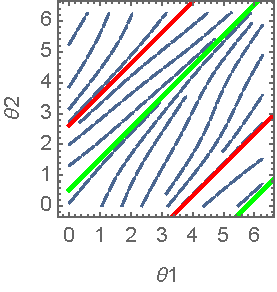
\includegraphics{img/C21thetaphaseportrait.pdf}

\vspace{0.2cm}

\hrule
\vspace{0.2cm}

\noindent\textbf{Big picture}

Simple nonlinear dynamical systems in 3 variables can have surprisingly complicated and hard to predict long term behavior.  The Lorenz '63 system is an important example of such a system: it is the system in which this kind of hard-to-predict behavior was first characterized.


\vspace{0.2cm}
\hrule
\vspace{0.2cm}

\noindent \textbf{Extra vocabulary / extra facts:}
\begin{tcolorbox}

A dynamical system is \textbf{dissipative} if volumes (or areas) in phase space are decreased under the forward action of the flow (for all forward times).  For physical systems, dissipation is associated with energy loss.

A dynamical system is \textbf{volume contracting} when the surface, $\partial V$, of a region $V$ moves under the action of the flow in such a way that the enclosed volume decreases with time. %A patch of surface sweeps out the volume $dA(\underline{f}\cdot\underline{n}dt$ in time $dt$.  We have $V(t+dt) = V(t)+\int_S\underline{f} dt\cdot\underline{n}\ dA$ so $\dot V = \frac{V(t+dt)-V(t)}{dt} = \int_S \underline{f}\cdot\underline{n}dA = \int_V \nabla\cdot \underline{f} dV$ by the divergence theorem.

When the \textbf{divergence} of the vector field is negative everywhere, volumes will be contracted by the flow.  \emph{See section 9.2 for details}.

In a dynamical system in 3d, \textbf{closed trajectories can be saddle-like}: they can have two spiraling directions that are stable and one non-spiraling direction that is unstable.  Or they might have two spiraling directions that are unstable and one that is stable.
\end{tcolorbox}

\begin{tcolorbox}
When a dynamical system is volume contracting, it will not have repelling fixed points or repelling limit cycles.  Those would create small regions of volume expansion.  Limit cycles and fixed points will be stable or saddle-type.

A dynamical system in $n$-dimensions has $n$ different \textbf{Lyapunov exponents}. Imagine creating a tiny (infinitesimal) sphere of perturbed initial conditions at a point in the phase space.  The Lyapunov exponents describe the evolution of the sphere into an ellipsoid under the local action of the flow.  In the Lorenz system the sphere is squished in some directions (negative Lyapunov exponents) and stretched in one direction (positive Lyapunov exponent).

Often the term \textbf{Lyapunov exponent} is used to refer to the largest one.

\end{tcolorbox}

\begin{tcolorbox}
\textbf{Some properties of the Lorenz '63 system}

\begin{align*}
\dot x &= -\sigma x + \sigma y \\
\dot y &= rx - y - xz \\
\dot z &= xy - bz
\end{align*}

This system has just two \textbf{quadratic nonlinearities} in the equations ($-xz$ and $xy$).

There is a spherical \textbf{trapping region}, $x^2+y^2 + (z-r-\sigma)^2 = C$ (for $C$ sufficiently large) and all trajectories eventually enter it. 

This system is (strongly) \textbf{volume contracting}.

Two trajectories that start very close to each other will \textbf{diverge}, separating exponentially fast.
\end{tcolorbox}

\begin{tcolorbox}
\textbf{Chaos} is aperiodic long term behavior that occurs in a deterministic system exhibiting senstive dependence on initial conditions.  See our text for more.  We'll ask for the following three ``ingredients'':
\begin{itemize}
    \item We can find trajectories that don't ``settle down'' to a fixed point, periodic orbit, or quasiperiodic orbit (aperiodic long term behavior).
    \item The system does not have random inputs: it is deterministic.
    \item Nearby trajectories separate exponentially fast (in the short term), so the system has a positive Lyapunov exponent.
\end{itemize}
An \textbf{attractor} is a closed set $A$ that is 
\begin{itemize}
    \item invariant: trajectories that start in $A$ stay in $A$ for all time.
    \item attracting: there is an open set (call it $U$) that contains $A$, and if we start at a point in $U$, $\underline{x}(0)$, its distance from $A$ will tend to zero as $t\rightarrow \infty$.
    \item minimal: there is no proper subset of $A$ that satisfies the two conditions above.
\end{itemize}
The \textbf{basin of attraction} of an attractor $A$ is the largest open set $U$ for which $A$ is attracting.
\end{tcolorbox}

\vspace{0.2cm}
\hrule
\vspace{0.2cm}

\textbf{Addressing your questions}
\begin{enumerate}
    \item Returning to timing of the limit cycle in the homoclinic bifurcation: $\mathcal{O}(\ln \mu)$ vs $T\propto \ln \frac{1}{\mu}$
    \item What was Steve's argument about quasiperiodicity and a torus?
    \item Steve mentioned that we never truly know where we are starting.  Wasn't this true in 2D as well?
    \item When we linearize, we just dropped the quadratic terms.  Is this equivalent to finding the Jacobian?  When can we do this?
        \item Steve looked only at $\dot x$ and $\dot y$.  Will we sometimes need a Jacobian for all three variables?
        \item With the Hopf bifurcation, how was its parameter value determined and how do we know it was subcritical?
        \item What happens to the system at large $r$?
    \item What does this strange attractor mean?
    \item How does the Lorenz system relate to other chaotic systems?
    \item What if the symmetry were removed from this system?  Could there still be chaotic behavior?
    \item Which parameters in the Rayleigh-Benard system affect what conditions?

    
\end{enumerate}

\vspace{0.2cm}
\hrule
\vspace{0.2cm}


\noindent\textbf{Skill Check C23 practice}
\begin{questions}
\item Retake of skill check C20: 

\item Find the Jacobian for the system $\dot x = -y-z, \dot y = x + ay, \dot z = b + z(x-c).$

\end{questions}

\vspace{0.2cm}

\hrule
\vspace{0.2cm}

\noindent\textbf{Skill check C23 practice solution}

Finding the partials (first row is partials of $\dot x$, second row is partials of $\dot y$, and third row is partials of $\dot z$).

$\left(\begin{array}{c c c} 0 & -1 & -1 \\ 1 & a & 0 \\ z & 0 & x-c\end{array}\right)$

\vspace{0.2cm}

\hrule
\vspace{0.2cm}
\noindent\textbf{Questions}

\noindent \ \ 0.  Share your sports/athletics preferences (either to participate or spectate) and write your names on the slide.

\begin{questions}





\item (Volume contraction) The Lorenz system is dissipative, meaning that volumes in the phase space are contracted under the flow.  Consider an arbitrary closed surface $S$.  This surface encloses a region $W$ that has volume $V$.  We can think of every point in $W$ as the initial condition of a trajectory.  Let each of them evolve forward in time (under the action of the dynamical system), let $W(t)$ be the set they evolve to at time $t$ (with surface $S(t)$.  The volume of the set is evolving in time!

%for time $\Delta t$, then the volume may change.  

How does the volume change with time?  

The divergence of a vector field is a measure of local contraction (negative sign) or local expansion (positive sign) under the action of the vector field.

The divergence theorem tells us that if we integrate the divergence over a region $W$, we learn about the net push of the vector field at the surface of the region.  

The action of the vector field is changing the size of our region.  For the size to change, the surface must be enclosing a growing or a shrinking volume.

Learning about the net push of the vector field at the surface tells us about the change in the volume.

Specifically:

$\displaystyle \dot{V} = \int_W \text{div }\vec{f}\ dV$ where $\vec f$ is the vector field given by the dynamical system.  
\begin{parts}
\item Find $\text{div }\vec f$ and argue that $\dot{V}$ is negative for the Lorenz system.  Use this to conclude that volumes contract.  When volumes in phase space are contracted under the action of the flow, we call a system \emph{dissipative}, so you are showing that the Lorenz system is a dissipative system.

\emph{Recall that $\text{div }\vec f = \nabla \cdot \vec f = \frac{\partial \dot x}{\partial x} + \frac{\partial \dot y}{\partial y} + \frac{\partial \dot z}{\partial z}$.}

\item Use $\dot V = \int_W \nabla \cdot \underline{f}\ dV$ to find $V(t)$ for this system.

\end{parts}

\question The characteristic equation for the eigenvalues of the Jacobian at the fixed points $C_+$ and $C_-$ is
\[\lambda^3 + (\sigma + b + 1)\lambda^2 + (r+\sigma) b \lambda + 2 b \sigma (r-1) = 0.\]

At the Hopf bifurcation, there is a pair of imaginary eigenvalues, $\lambda_+ = i\omega$ and $\lambda_- = -i\omega$.
There must be a third eigenvalue, too, $\lambda_3$.  By assuming all three of these eigenvalues are solutions of the characteristic equation, meaning that they
are roots of the polynomial equation, find $\lambda_3$ and construct an implicit relationship for $r_H$, the value of $r$ at the Hopf.

\question Show that the $z$-axis is an invariant line of the Lorenz equations, so a trajectory that starts on the axis stays on the axis.

\item I'm providing Mathematica code for you to explore the Lorenz system and the Rossler system.
\begin{parts}
\part Try different values of $r$ for the Lorenz system (both bigger and smaller) and use them to plot trajectories in the phase space and vs time.  Perhaps look up some interesting values.  
\part Read the code for the Poincar\'e map, and look up any commands that aren't familiar.  Work to figure out what is going on with this code.  Add axis labels to the plot to represent what it is showing.
\part Do the same for the z-``map''.  What does this seem to be showing?  This map is called the Lorenz map.
\part Explore these for the Rossler system.
\end{parts}

\end{questions}

\eject
1a: $\vec\nabla \cdot \vec f = -\sigma -1 -b < 0$.  This is a constant, so $\dot V = -(\sigma + 1 + b)\int_W dV = -(\sigma + 1 + b)V$. 1b: $\dot V = -(\sigma + 1 + b)V$ so $V(t) = V_0 e^{-(\sigma+1+b)t}.$

2: Close to the Hopf bifurcations, the eigenvalues will be of the from $a - i\omega, a + i\omega, \lambda_3$.  At the bifurcation itself, $a = 0$.

A characteristic equation with these roots is:
$(\lambda - i\omega)(\lambda+i\omega)(\lambda-\lambda_3) = 0$

At $r = r_H$ we have $\lambda^3 - \lambda_3 \lambda^2 + \omega^2 \lambda - \omega^2\lambda_3 = 0$.

Matching terms: $\lambda_3 = -(\sigma + b +1)$.  $\omega^2 = (r+\sigma)b$.  

An implicit equation for $r_H$ at the moment of bifurcation can be found from setting $-\omega^2\lambda_3 = 2b\sigma(r-1)$ given the expressions for $\omega^2$ and $\lambda_3$ above, so 

$(\sigma+b+1)b(r_H+\sigma) = 2b\sigma(r_H-1)$

3. On this line $x = 0$ and $y=0$ so $\dot x = \sigma(0-0) = 0$.  $\dot y = r(0)-0-0(z) = 0$.  $\dot x = 0$ and $\dot y = 0$ so if we start on the line we can't leave the line.
\end{document}